\documentclass[12pt]{article}
\usepackage{multicol} %multicolumns
\usepackage{siunitx} %log table stuff
\usepackage{flafter}
\usepackage{amsmath} %math stuff
\usepackage{amssymb} %math symbols
\usepackage{graphicx} %including photos
\usepackage{wrapfig} %for wrapping figure
%\graphicspath{{./Report For Titanium Doping/}} %path of folder from where photo needs to be extracted, NOT NECESSARY AT ALL TIMES
\usepackage[utf8]{inputenc}
\usepackage{float} %Using [H] command to stop picturefloating around
\usepackage{enumerate} %changing labels of lists
\usepackage{fancyhdr}
\usepackage{dsfont} %for set notations and other fancy letters
\usepackage{mathrsfs}
\usepackage[compat=1.0.0]{tikz-feynman}

\usepackage{geometry}
\geometry{
a4paper,
total={170mm,257mm},
top=20mm,
}
\usepackage{array}
\setlength\extrarowheight{4pt}
%\usepackage[dvipsnames]{xcolor} %for using coloured text
\usepackage{longtable,pdflscape,booktabs} % long table stuff
\usepackage{lscape} 
\usepackage{caption}
\captionsetup{labelformat=empty}
\captionsetup[subfigure]{labelformat=empty}
\usepackage{subcaption}
\usepackage{setspace} %for desired spacing between lines
\usepackage{blindtext} % for blind text in contents page
\usepackage[normalem]{ulem} %dash and dotted underline
\usepackage{bm} % for bold math symbols- using command \boldsymbol
\usepackage{mathtools} %for rcases
\usepackage{hyperref} %for hyperlinks
\usepackage{romannum} %for Roman Numerals
\usepackage[makeroom]{cancel} % for striked out or other stuff in math environment
\usepackage{tikz}
\usepackage{empheq} %  fancy math stuff
\usepackage{xfrac}
\usepackage{fancybox} %for fancy boxes
\usepackage{circuitikz}
\usepackage{listings}

\allowdisplaybreaks
\colorlet{linkequation}{blue} %making coloured equation refernces

\usetikzlibrary{shadows} %defines shadows
\usepackage[framemethod=tikz]{mdframed}
\usepackage{tcolorbox} %coloured boxes

\tikzset{rndblock/.style={rounded corners,rectangle,draw,outer sep=1pt,inner sep=5pt,line width=1pt}}

% Command Definition
% 1 optional to customize the aspect, 2 mandatory: text to be framed
\newcommand{\mybox}[2][]{\tikz[baseline=(h.base)]\node[rndblock,#1] (h) {#2};}

%definining new command to make coloured equation references
\newcommand*{\myref}[1]{%
  \begingroup
    \hypersetup{
      linkcolor=linkequation,
      linkbordercolor=linkequation,
    }%
    \ref{#1}%
  \endgroup
}

%Setting equations a particular colour
\hypersetup{
colorlinks=true,
linkcolor=black,
filecolor=magenta,
urlcolor=Black,
citecolor=blue,
}

\parskip 1ex

%For circled numbers
\newcommand*\circled[1]{\tikz[baseline=(char.base)]{
            \node[shape=circle,draw,inner sep=2pt] (char) {#1};}}
            
%command for making capital roman numerals
%\newcommand{\RomanNum}[1]{\MakeUppercase{\romannumeral #1}}

%%%%%%%%%%%%%%%%%%%%%%%%%%%%%%%%%%%%%%%%%%%%%%%%%%%%%%%%%%%%%%%%%%%%%%%%%%%%%%%%%%%%%%%%%%%%%%%%%%%%%%%%%%%%%%%%%%%%%%%%%%%%%%%%%%%%%%%%%%%%%%%%%%%%%%%%%%%%%%%%%%%%%%%%%%%%%%%%%%%%%%%%%%%%% DOCUMENT BEGINS %%%%%%%%%%%%%%%%%%%%%%%%%%%%%%%%%%


%\pagestyle{fancy}
%\fancyhf{}
%\fancyhead[LO]{\rightmark}
%\fancyhead[RE]{\leftmark}

\usepackage{titlesec, blindtext}
\titleformat{\section}[hang]{\Huge\bfseries}{\Roman{section}. \hspace{20pt}}{0pt}{\Huge\bfseries}

\titleformat*{\subsection}{\Large\bfseries}
\titleformat*{\subsubsection}{\large\bfseries}

\usepackage{tocloft}
\renewcommand{\cftsecleader}{\cftdotfill{\cftdotsep}}
\renewcommand{\cftsecaftersnum}{.}%

%%%%%%%%%%%%%%%%%%%%%%%%%%%%%%%%%%%%%%%%
\definecolor{codegreen}{rgb}{0,0.6,0}
\definecolor{codegray}{rgb}{0.5,0.5,0.5}
\definecolor{codepurple}{rgb}{0.58,0,0.82}
\definecolor{backcolour}{rgb}{0.95,0.95,0.92}

\lstdefinestyle{mystyle}{
    backgroundcolor=\color{backcolour},   
    commentstyle=\color{codegreen},
    keywordstyle=\color{magenta},
    numberstyle=\tiny\color{codegray},
    stringstyle=\color{codepurple},
    basicstyle=\ttfamily\footnotesize,
    breakatwhitespace=false,         
    breaklines=true,                 
    captionpos=b,                    
    keepspaces=true,                 
    numbers=left,                    
    numbersep=5pt,                  
    showspaces=false,                
    showstringspaces=false,
    showtabs=false,                  
    tabsize=2
}

\lstset{style=mystyle}
%%%%%%%%%%%%%%%%%%%%%%%%%%%%%%%%%%%%%%%%%%%%%%%%%%

\begin{document}
\doublespace
%making the title page
\pagenumbering{gobble}
\begin{titlepage}
	\begin{center}
		\vspace*{0.2cm}
		\textbf{\uline{P441/P442 - Open Lab Experiment}} \linebreak
		\vspace{1.5cm}\linebreak
		\textbf{\Large{NON-LINEAR DYNAMICS CIRCUIT}}\linebreak
		\vspace{2cm} \linebreak
		\textit{Submitted By} \linebreak \textbf{ASHMITA PANDA} \linebreak 
		\textbf{ROLL NO. 1811042} \linebreak
		School of Physical Sciences \linebreak National Institute of Science, Education and Research (NISER), Bhubaneswar \linebreak
		Date of Submission : 24\textsuperscript{th} September, 2021
		\vspace{2.5cm} \linebreak
		\textit{Under the Guidance of} \linebreak \textbf{Dr. Pratap Kumar Sahoo} \linebreak Associate Professor \linebreak School of Physical Sciences \linebreak National Institute of Science Education and Research (NISER), Bhubaneswar
		\vspace{1cm} \linebreak

	\end{center}
	\begin{figure}[H]
		\centering
		
\includegraphics[width=0.17\textwidth]{niser logo}
	\end{figure}
\end{titlepage}

\raggedright
\newpage
\pagenumbering{roman}

\singlespacing
%Table of Contents
\tableofcontents
\addtocontents{toc}{~ \hfill \textbf{Page} \par}
\onehalfspacing

\newpage
\pagenumbering{arabic}
\begin{center}
	\textbf{\Large Abstract} \linebreak
	\blindtext[0]
\end{center}
\rule{17cm}{1pt}

% SECTION - INTRODUCTION
\section{Introduction}
Chua circuit is the simplest electronic circuit which exhibits the phenomenon of chaos. It was invented by Leon Chua in 1983.
\linebreak

A dynamical system is said to have chaotic behaviour when despite its deterministic nature, it is not predictable. The apparent random behaviour of the system is usually governed by deterministic laws that are highly sensitive to initial conditions. A small change in initial conditions can result in widely varying results.
\linebreak

To exhibit chaos, a circuit must have been :
\begin{enumerate}[i.)]
	\item at least one locally active resistor
	\item at least one non-linear element
	\item at least three energy storage units
\end{enumerate}
%%%%%%%%%%%%%%%%%%%%%%%%%%%%%%%%%%%%%%%%%%%%%%%%%%%%%%%%%%%
%SECTION 1 - THEORETICAL DESIGN
\section{Theoretical Design}
%subsection 2.1 - Circut elements and constraints
\subsection{Circuit Elements and Constraints}
In order to physically exhibit the phenomenon of chaos Chua decided to design a physical circuit with 3 unstable equilibrium points with further contraints that number of passive elements should be as few as possible and there should be only one non-linear resistor with two terminals which has piecewise linear characteristic. \linebreak

There must be 3 energy storage elements as the dynamical system must have at least order 3 to be chaotic. He also decided to have only one passive element in the circuit - a linear resistor. \linebreak
Passive elements are the circuit elements which donot generate power but instead store or dissipate it. \linebreak

Also since we want to observe oscillations, we cannot have only capacitors or only inductors as all 3 energy storage elements. There must be some combination of both. Chua preferred the combination of two capacitors and one inductor to make the circuit more cost-efficient. 
%
%subsection 2.2 - Possible Confugurations
\subsection{Possible Configurations}
With these constraints in place, there can be 8 possible configurations. 
\begin{figure}[H] %possible circuits
	\centering
	\caption{Fig 1. Possible configurations for the circuit}
	% a and b
	\begin{subfigure}[b]{0.5\textwidth}
		\centering
		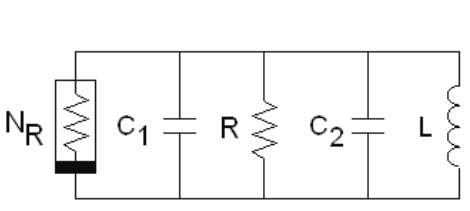
\includegraphics[width=0.9\textwidth]{Images/fig1(a).png}
		\caption{(a)}
		\label{fig:1a}
	\end{subfigure}%
	\begin{subfigure}[b]{0.5\textwidth}
		\centering
		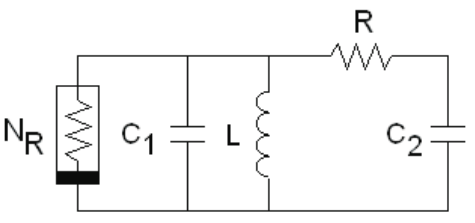
\includegraphics[width=0.9\textwidth]{Images/fig1(b).png}
		\caption{(b)}
		\label{fig:1b}
	\end{subfigure}
	% c and d
	\begin{subfigure}[b]{0.5\textwidth}
		\centering
		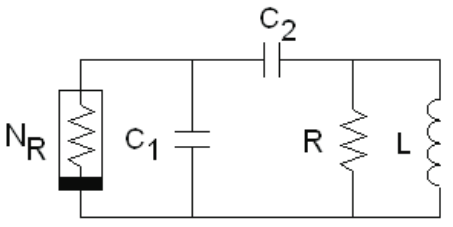
\includegraphics[width=0.9\textwidth]{Images/fig1(c).png}
		\caption{(c)}
		\label{fig:1c}
	\end{subfigure}%
	\begin{subfigure}[b]{0.5\textwidth}
		\centering
		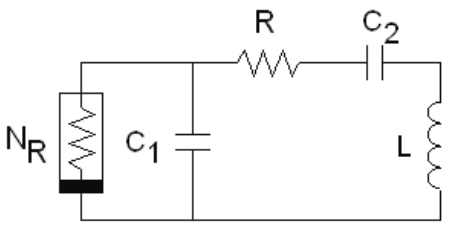
\includegraphics[width=0.9\textwidth]{Images/fig1(d).png}
		\caption{(d)}
		\label{fig:1d}
	\end{subfigure}
	% e and f
	\begin{subfigure}[b]{0.5\textwidth}
		\centering
		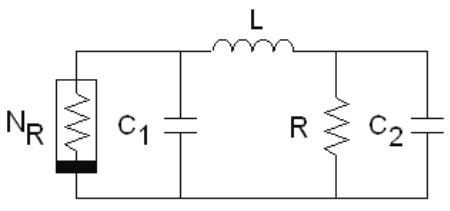
\includegraphics[width=0.9\textwidth]{Images/fig1(e).png}
		\caption{(e)}
		\label{fig:1e}
	\end{subfigure}%
	\begin{subfigure}[b]{0.5\textwidth}
		\centering
		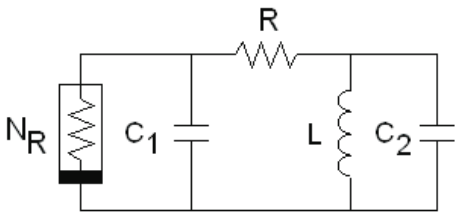
\includegraphics[width=0.9\textwidth]{Images/fig1(f).png}
		\caption{(f)}
		\label{fig:1f}
	\end{subfigure}
\end{figure}
\begin{figure}[H]
	\centering
	\caption{Fig 1. Possible configurations for circuit}
	% g and h
	\begin{subfigure}[b]{0.5\textwidth}
		\centering
		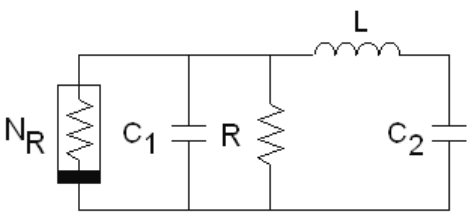
\includegraphics[width=0.9\textwidth]{Images/fig1(g).png}
		\caption{(g)}
		\label{fig:1g}
	\end{subfigure}%
	\begin{subfigure}[b]{0.5\textwidth}
		\centering
		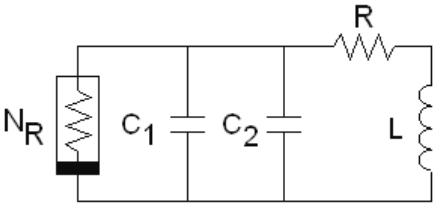
\includegraphics[width=0.9\textwidth]{Images/fig1(h).png}
		\caption{(h)}
		\label{fig:1h}
	\end{subfigure}
\end{figure}
Configuration (g) and (h) can be immediately rejected. \linebreak
In (g) the characteristic of resistance R can be absorbed in the characteristics of non-linear resistor $N_R$.
In (h) the $C_1$ and $C_2$ capacitances can be replaced by a single effective capacitor $C=C_1+C_2$. 
So in both of these configurations all circuit elements donot give unique contribution. Thus they can be rejected.\linebreak

For (a) and (b), the DC equilibrium calculations show that non-linear resistor gets short-circuited by the inductor. 
For (c) and (d), the DC equilibrium calculations show that non-linear resistor terminals are open.
So all the four configurations can be rejected. \linebreak

The remaining configuration (e) and (f) are both valid, but Chua selected configuration (f) because the RLC subcircuit generates oscillations.
%
%subsection 2.3
\subsection{Final Circuit}
The final Chua circuit is given as follows :
\begin{figure}[H]
	\centering
	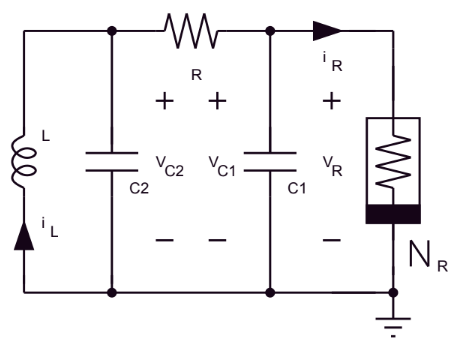
\includegraphics[width=0.6\textwidth]{Images/fig2_final.png}
	\caption{Fig 2. Chua's Circuit}
\end{figure}
%
%%%%%%%%%%%%%%%%%%%%%%%%%%%%%%%%%%%%%%%%%%%%%%%%%%%%%%%%%%%%
% SECTION 3 - STATE EQUATIONS AND SIMULATION
\section{State Equations and Simulations}
%subsection 3.1
\subsection{State Equations}
The equations of Chua's circuit are given as a system of three coupled differential equations :
\begin{align}
	C_1 \dfrac{dv_{C_1}}{dt}&=G\left( v_{C_2}-v_{C_1} \right)-g(v_{C_1}) \label{eq:1} \\
	C_2 \dfrac{dv_{C_2}}{dt}&=G\left( v_{C_1}-v_{C_2} \right)-i_L \label{eq:2}\\
	L \dfrac{i_L}{dt}&=-v_{C_2}\label{eq:3}
\end{align}
where, $G=\dfrac{1}{R}$ is the conductance, and $g(x)$ is a piece-wise linear function. It is given as :
\begin{align}
	g(x)&=m_0x+\dfrac{1}{2}(m_1-m_0)\left[ |x+B_p|-|x-B_p| \right] \label{eq:4}
\end{align}
where,
\begin{align*}
	m_0 &\implies \text{slope of outer region} \\
	m_1 &\implies \text{slope of inner region} \\
	B_P &\implies \text{breakpoints (both positive and negative values)}
\end{align*}
%
%subsection 3.2 - simulations
\subsection{Simulation}
The variables were redefined and all constants were taken to right hand side to make handling the equations easier.
\begin{align}
	\dfrac{dx}{dt}&=\dfrac{1}{C_1}\left\{ G\left( y-x \right)-g(x) \right\} \label{eq:5} \\
	\dfrac{dy}{dt}&=\dfrac{1}{C_2}\left\{ G\left( x-y \right)-z \right\} \label{eq:6} \\
	\dfrac{dz}{dt}&=-\dfrac{y}{L} \label{eq:7}
\end{align}
where,
\[ x \equiv v_{C_1} \quad y \equiv v_{C_2} \quad z \equiv i_L \]
The equation $g(x)$ remains the same as in (\myref{eq:4}).\linebreak
The equations are solved numerically using Runge Kutta 4 method in Python. All plots are made using Gnuplot.
%
%subsubsection 3.2.1 - Pyhton
\subsubsection{Python Codes}
The code for RK4 is as follows :
\lstinputlisting[language=Python]{/home/ashmita/Desktop/ASHMITA/APanda_Lib/chua_circuit_simulations.py}
The code inputs the three differential equations as a column vector F which is a function of x, y, z and t (time). x, y and z are arranged as column vector b. For the first iterations, it has the initial values. 
h is the increment factor. N is the number of iterations. $t_0$ is the initial time value. \linebreak

The `append.file()' function saves the data points (t, x, y and z) after each iteration in a file (filename provided to function as variable `name'). All codes for manipulation with files is as follows :
\lstinputlisting[language=Python]{/home/ashmita/Desktop/ASHMITA/APanda_Lib/handling_files.py}
%
% subsubsection 3.2.2 - plots with dimensionless constants
\subsubsection{Plots with Dimensionless Constants}
The following values were used for the constants :
\[ G=0.7 \quad C_1=1/9 \quad C_2=1 \quad L=1/7 \quad B_p=1 \quad m_0=-0.5 \quad m_1=-0.8 \]
The code for defining the function, initial values and calling the function is :
\lstinputlisting[language=Python]{/home/ashmita/Desktop/ASHMITA/NISER Study/7th Semester/Open Lab/Non-Linear Circuit/Dimensionless/dimensionless_chua.py}



\end{document}
